%package list
\documentclass{article}
\usepackage[top=3cm, bottom=3cm, outer=3cm, inner=3cm]{geometry}
\usepackage{graphicx}
\usepackage{url}

%% \usepackage{cite}
\usepackage{hyperref}
\usepackage{array}
\usepackage{multicol}
\newcolumntype{x}[1]{>{\centering\arraybackslash\hspace{0pt}}p{#1}}
\usepackage{natbib}
\usepackage{pdfpages}
\usepackage{multirow}
\usepackage{float}
\usepackage[normalem]{ulem}
\useunder{\uline}{\ul}{}


%%%%%%%%%%%%%%%%%%%%%%%%%%%%%%%%%%%%%%%%%%%%%%%%%%%%%%%%%%%%%%%%%%%%%%%%%%%%
%%%%%%%%%%%%%%%%%%%%%%%%%%%%%%%%%%%%%%%%%%%%%%%%%%%%%%%%%%%%%%%%%%%%%%%%%%%%
\newcommand{\csemail}{vmachacaa@unsa.edu.pe}
\newcommand{\csdocente}{Vicente Machaca Arceda}
\newcommand{\cscurso}{Algoritmos y Estructura de Datos}
\newcommand{\csuniversidad}{Universidad Nacional de San Agustín}
\newcommand{\csescuela}{Maestría en Ciencia de la Computación}
\newcommand{\cspracnr}{01}
\newcommand{\cstema}{--}
%%%%%%%%%%%%%%%%%%%%%%%%%%%%%%%%%%%%%%%%%%%%%%%%%%%%%%%%%%%%%%%%%%%%%%%%%%%%
%%%%%%%%%%%%%%%%%%%%%%%%%%%%%%%%%%%%%%%%%%%%%%%%%%%%%%%%%%%%%%%%%%%%%%%%%%%%


\usepackage[english,spanish]{babel}
\usepackage[utf8]{inputenc}
\AtBeginDocument{\selectlanguage{spanish}}
\renewcommand{\figurename}{Figura}
\renewcommand{\refname}{Referencias}
\renewcommand{\tablename}{Tabla} %esto no funciona cuando se usa babel
\AtBeginDocument{%
	\renewcommand\tablename{Tabla}
}

\usepackage{fancyhdr}
\pagestyle{fancy}
\fancyhf{}
\setlength{\headheight}{30pt}
\renewcommand{\headrulewidth}{1pt}
\renewcommand{\footrulewidth}{1pt}
\fancyhead[L]{\raisebox{-0.2\height}{
\includegraphics[width=3cm]{img/logo_unsa}}}
\fancyhead[C]{}
\fancyhead[R]{\fontsize{7}{7}\selectfont	\csuniversidad \\ \csescuela \\ \textbf{\cscurso} }
\fancyfoot[L]{MSc. Vicente Machaca}
\fancyfoot[C]{\cscurso}
\fancyfoot[R]{Página \thepage}

\begin{document}
	
	\vspace*{10px}
	
	\begin{center}	
		\fontsize{17}{17} \textbf{ Práctica \cspracnr}
	\end{center}
	%\centerline{\textbf{\underline{\Large Título: Informe de revisión del estado del arte}}}
	%\vspace*{0.5cm}
	

	\begin{table}[h]
		\begin{tabular}{|x{4.7cm}|x{4.8cm}|x{4.8cm}|}
			\hline 
			\textbf{DOCENTE} & \textbf{CARRERA}  & \textbf{CURSO}   \\
			\hline 
			\csdocente & \csescuela & \cscurso    \\
			\hline 
		\end{tabular}
	\end{table}	
	
	
	\begin{table}[h]
		\begin{tabular}{|x{4.7cm}|x{4.8cm}|x{4.8cm}|}
			\hline 
			\textbf{PRÁCTICA} & \textbf{TEMA}  & \textbf{DURACIÓN}   \\
			\hline 
			\cspracnr & Algoritmos de Ordenamiento & 3 horas   \\
			\hline 
		\end{tabular}
	\end{table}
	
	
	\section{Datos de los estudiantes}
	\begin{itemize}
		\item Grupo: V
		\item Integrantes: 
		\begin{itemize}
			\item Angel Yvan Choquehuanca Peraltilla
			\item Estefany Pilar Huaman Colque
            \item Eduardo Diaz Huayhuas
            \item Gustavo Raul Manrique Fernandez
		\end{itemize}		
	\end{itemize}
	
	
 
	


	%\clearpage
	%\bibliographystyle{apalike}
	%\bibliographystyle{IEEEtranN}
	%\bibliography{bibliography}
		

    \section{Introducción}
    Se considera un algoritmo de ordenamiento a un conjunto de ordenes que permite que: A un vector o conjunto de datos se le aplique acciones de reordenamiento. Este algoritmo puede ser de diferente tipo de secuencias con el mismo fin. 

    Desde la aparición del primer algoritmo (BubbleSort en 1956), la formulación de algoritmos viene siendo un caso de estudio por cientificos afines a la materia.

    Con el pasar de los años se ha clasificado los algoritmos de acuerdo al metodo de ordenamiento.
    En este informe se aborda el analisis de tiempo en ejecución de diferentes algoritmos en los lenguajes Python, C++ y Go.

    \section{Marco Teorico}
    \subsection{Merge Sort}
    \paragraph{ Concepto}El algoritmo de ordenamiento por mezcla (merge sort en inglés) es un algoritmo de ordenamiento externo estable basado en la técnica divide y vencerás. La idea de los algoritmos de ordenación por mezcla es dividir la matriz por la mitad una y otra vez hasta que cada pieza tenga solo un elemento de longitud. Luego esos elementos se vuelven a juntar (mezclados) en orden de clasificación.

    \paragraph{Ejemplo:}
    \paragraph{Fase 1:} Para 8 datos
    \begin{enumerate}
        \item Comenzamos dividiendo la matriz: [31,4,88,2,4,2,42]
        \item Dividimos en 2 partes: [31,4,88,1][4,2,42]
        \item Dividimos en 4 partes: [31,4] [88,1] [4,2] [42] 
        \item Luego en piezas individuales: [31][4][88][1][4][2][42]
    \end{enumerate}
    \paragraph{Fase 2:} Ahora tenemos que unirlos de nuevo en orden de mezcla
\begin{enumerate}
    \item Primero fusianamos elementos individuales en pares. Cada par se fusiona en orden de mezcla: [4,31] [1,88] [2,4] [42]
    \item Luego fusionamos los pares en orden de mezcla: [1,4,31,88] [2,4,42]
    \item Y luego fusionamos los dos últimos grupos. [1,2,4,4,31,42,88]
\end{enumerate}    
    
    \subsection{Tree Sort}
    
     Tree sort es un algoritmo de ordenación que crea un árbol de búsqueda binaria a partir de los elementos que se van a ordenar y luego atraviesa el árbol ( en orden ) para que los elementos aparezcan ordenados. [1] Su uso típico es ordenar elementos en línea 
     
     Este ordenamiento trabaja de la siguiente manera:
     \begin{itemize}
            \item Compara el valor a almacenar con el primer nodo del árbol, si este es menor al valor del nodo, entonces se evalúa el nodo izquierdo, de lo contrario se evalúa el nodo derecho siguiendo la misma regla hasta no encontrar más nodos que evaluar..

            \item Si el nodo izquierdo o derecho estuvieran vacíos, esa será la posición final del valor, por lo que crearemos un nuevo nodo en esta ubicación y almacenaremos el valor.
            
            \item Una vez que todos los valores se encuentran almacenados en sus respectivas posiciones, procedemos a recuperar los valores de cada nodo haciendo un recorrido inorden, el cuál consiste en procesar primero la rama izquierda, luego el valor actual y después la rama derecha de cada nodo.
    Por ejemplo en la siguiente Figura se observa una demostración de la estructura:
        
        \end{itemize}
        
\begin{figure}[H]
\centering
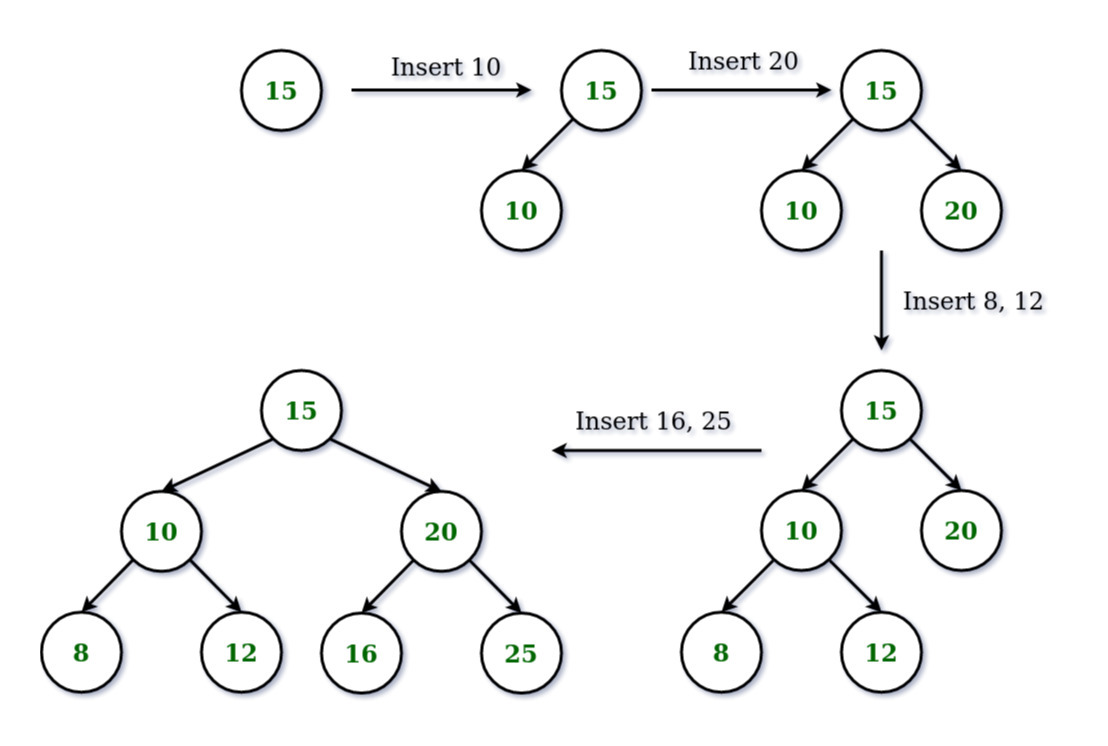
\includegraphics[width=0.9\textwidth]{img/treeejem.jpg}
\caption{Ordenamiento TreeSort}
\label{fig:QuickSort}
\end{figure}

	\subsection{Quick Sort}
	El algoritmo trabaja de la siguiente forma:
	\begin{itemize}
		\item Elegir un elemento del conjunto de elementos a ordenar, al que llamaremos pivote.
		\item Resituar los demás elementos de la lista a cada lado del pivote, de manera que a un lado queden todos los menores que él, y al otro los mayores. Los elementos iguales al pivote pueden ser colocados tanto a su derecha como a su izquierda, dependiendo de la implementación deseada. En este momento, el pivote ocupa exactamente el lugar que le corresponderá en la lista ordenada.
		\item La lista queda separada en dos sublistas, una formada por los elementos a la izquierda del pivote, y otra por los elementos a su derecha.
		Repetir este proceso de forma recursiva para cada sublista mientras éstas contengan más de un elemento. Una vez terminado este proceso todos los elementos estarán ordenados.
		Como se puede suponer, la eficiencia del algoritmo depende de la posición en la que termine el pivote elegido.
		
		\item En el mejor caso, el pivote termina en el centro de la lista, dividiéndola en dos sublistas de igual tamaño. En este caso, el orden de complejidad del algoritmo es O(n·log n).
		\item En el peor caso, el pivote termina en un extremo de la lista. El orden de complejidad del algoritmo es entonces de O(n²). El peor caso dependerá de la implementación del algoritmo, aunque habitualmente ocurre en listas que se encuentran ordenadas, o casi ordenadas. Pero principalmente depende del pivote, si por ejemplo el algoritmo implementado toma como pivote siempre el primer elemento del array, y el array que le pasamos está ordenado, siempre va a generar a su izquierda un array vacío, lo que es ineficiente.
		\item En el caso promedio, el orden es O(n·log n).
		No es extraño, pues, que la mayoría de optimizaciones que se aplican al algoritmo se centren en la elección del pivote.
	\end{itemize}
	
	\subsection{Heap Sort}
	El ordenamiento por montículos (heapsort en inglés) es un algoritmo de ordenamiento no recursivo, no estable, con complejidad computacional O(n·log n).
	
	Este algoritmo consiste en almacenar todos los elementos del vector a ordenar en un montículo (heap), y luego extraer el nodo que queda como nodo raíz del montículo (cima) en sucesivas iteraciones obteniendo el conjunto ordenado. Basa su funcionamiento en una propiedad de los montículos, por la cual, la cima contiene siempre el menor elemento (o el mayor, según se haya definido el montículo) de todos los almacenados en él. El algoritmo, después de cada extracción, recoloca en el nodo raíz o cima, la última hoja por la derecha del último nivel. Lo cual destruye la propiedad heap del árbol. Pero, a continuación realiza un proceso de "descenso" del número insertado de forma que se elige a cada movimiento el mayor de sus dos hijos, con el que se intercambia. Este intercambio, realizado sucesivamente "hunde" el nodo en el árbol restaurando la propiedad montículo del árbol y dejando paso a la siguiente extracción del nodo raíz.
	
	El algoritmo, en su implementación habitual, tiene dos fases. Primero una fase de construcción de un montículo a partir del conjunto de elementos de entrada, y después, una fase de extracción sucesiva de la cima del montículo. La implementación del almacén de datos en el heap, pese a ser conceptualmente un árbol, puede realizarse en un vector de forma fácil. Cada nodo tiene dos hijos y por tanto, un nodo situado en la posición i del vector, tendrá a sus hijos en las posiciones 2 x i, y 2 x i +1 suponiendo que el primer elemento del vector tiene un índice = 1. Es decir, la cima ocupa la posición inicial del vector y sus dos hijos la posición segunda y tercera, y así, sucesivamente. Por tanto, en la fase de ordenación, el intercambio ocurre entre el primer elemento del vector (la raíz o cima del árbol, que es el mayor elemento del mismo) y el último elemento del vector que es la hoja más a la derecha en el último nivel. El árbol pierde una hoja y por tanto reduce su tamaño en un elemento. El vector definitivo y ordenado, empieza a construirse por el final y termina por el principio.

%\item Complejidad

 \begin{itemize}
          \item Complejidad temporal en el peor de los casos: $\Theta (n.log n)$  utilizando un árbol de búsqueda binario equilibrado; $\Theta (n^2)$ usando un árbol de búsqueda binario no balanceado.
           \item Complejidad de tiempo de caso promedio:$\Theta (n.log n)$
           \item Complejidad del tiempo en el mejor de los casos:$\Theta (n.log n)$
           \item Complejidad del espacio: $\Theta (n)$

\end{itemize}

    
    
    
    \section{Datos del Equipo}
    Para los algoritmos de mergesort y treesort se utilizó un equipo en la nube proporcionado por \href{https://replit.com/~}{www.replit.com}, con las siguientes caracteristicas:

    \begin{itemize}
        \item 0.5 vCPU con el sistema operativo Ubuntu 21.04-KVM
        \item 1 GB de Memoria RAM
        \item 1 TB de disco SSD
    \end{itemize}

	Para los algoritmos de heapsort y quicksort se utilizó una laptop con las siguientes caracteristicas:
	
	\begin{itemize}
		\item Intel Core i5-3230M @ 2.60 Hz
		\item Sistema operativo Windows 10 Pro
		\item 12 GB de Memoria RAM
		\item 292 GB de disco SSD
	\end{itemize}

    \section{Metodologia y Desarrollo}
    Para realizar las experiencias con mergesort y treesort tomaron en cuenta los siguientes aspectos:
    
    \begin{enumerate}
        \item Se preparó los datos a partir de un generador de valores en Python mediante la libreria \textit{random}. Estos valores son usados para los 3 lenguajes en su ejecución.
        \item Se subieron los archivos en la maquina virtual proporcionado por Replit.
        \item Se preparó el entorno de trabajo separado por carpetas e instalando los compiladores adecuados.
        \item Se utilizó el comando \textbf{time} de Linux para calcular el tiempo de ejecución real y del sistema.
        \item Se hace 5 pruebas por cada ejecución y se grabaron los resultados en una tupla en \textit{Google Colab}.
        \item Se hace uso de la libreria \textbf{MatPlotLib} de Python para la realización de los calculos estadisticos y graficos.
    \end{enumerate}
	Para realizar las experiencias con quicksort y heapsort tomaron en cuenta los siguientes aspectos:
	
	\begin{enumerate}
		\item Se generó valores aleatorios con Excel y se almacenó en archivos csv.
		\item Se preparó el entorno de trabajo separado por carpetas e instalando los compiladores adecuados.
		\item Se utilizó las librerías time de python, chrono de c++ y time de go para calcular el tiempo de ejecución real y del sistema.
		\item Se hace 5 pruebas por cada ejecución y se grabaron los resultados en un archivo csv.
		\item Se hace uso de la libreria \textbf{MatPlotLib} de Python para la realización de los calculos estadisticos y graficos.
	\end{enumerate}

\section{Resultados}
\subsection{Merge Sort} 
Se utilizó el comando time para generar el tiempo de compilacion para cada lenguaje. Todo estos datos fueron almacenados en una libreta Jupyter para posteriormente utilizar la libreria Matplotlib de Python para generar las graficas.
 Tambien se realizó calculos estadisticos utilizando la liberia Numpy. Los datos fueron almacenados y procesados para su respectiva tabla.

 
    \begin{figure}[H]
        \centering
        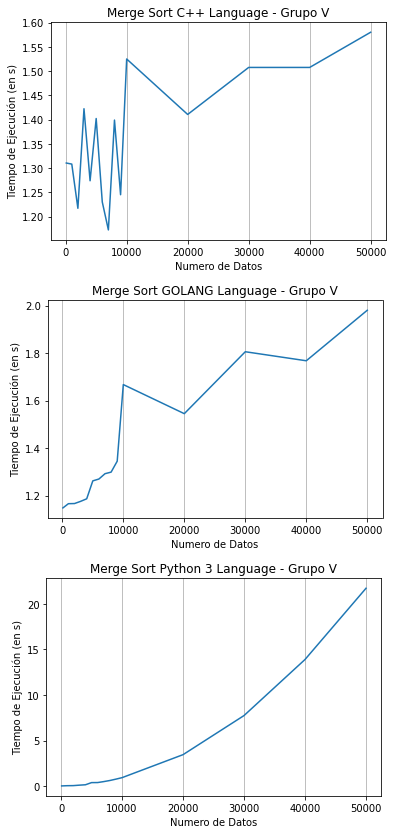
\includegraphics[scale=0.6]{img/finalmerg.png}
        \caption{Algoritmo MergeSort}
        \label{fig:my_label}
    \end{figure}

\begin{table}[H]
\begin{center}
\begin{tabular}{| c | c | c | c | c | c | c |}
\hline
\multicolumn{7}{ |c| }{Algoritmo MergeSort - Promedios y Desviacion Estandar} \\ \hline
Datos & C++ (s) & Go (s) & Py (s) &  DE C++ & DE Go & DE Py\\ \hline
100 & 1.3104 & 1.1484 & 0.0352 & 0.11226 & 0.07171 & 0.00444 \\
1000 & 1.3082 & 1.1662 & 0.0596 & 0.12914 & 0.03769 & 0.00417 \\
2000 & 1.217 & 1.1667 & 0.068 & 0.11981 & 0.03166 & 0.00572 \\
3000 & 1.4224 & 1.176 & 0.118 & 0.07406 & 0.03871 &  0.00993 \\
4000 & 1.2738 & 1.1868 & 0.1612 & 0.074405 & 0.017982 & 0.00495 \\
5000 & 1.4022 & 1.2622 & 0.3974 &  0.07954 & 0.01495 & 0.04623 \\
6000 & 1.23 & 1.27 & 0.4034 & 0.073759 & 0.02530 &  0.01382 \\
7000 & 1.1724 & 1.2924 & 0.5084 & 0.10504 & 0.01942 & 0.01861 \\
8000 & 1.3989 & 1.299 & 0.6282 & 0.10770 & 0.02265 & 0.03787 \\
9000 & 1.2449 & 1.345 & 0.7786 & 0.08257 & 0.02566 & 0.02032 \\
10000 & 1.525 & 1.6674 & 0.94 &  0.02795 & 0.06302 & 0.048985 \\
20000 & 1.4105 & 1.545 & 3.4601 & 0.10274 & 0.12826 &  0.1004 \\
30000 & 1.5076 & 1.8056 & 7.7452 &  0.07759 & 0.05421 & 0.176682 \\
40000 & 1.5076 & 1.7676 & 13.8876 & 0.07759 &  0.04846 & 0.66075 \\
50000 & 1.5802 & 1.9802 & 21.6906  & 0.03328  &  0.08478 & 0.71114 \\ \hline
\end{tabular}
\caption{Tiempo de Ejecución}
\label{tab:coches}
\end{center}
\end{table}

\subsection{Tree Sort}
Se utilizó el comando time para generar el tiempo de compilacion para cada lenguaje. Todo estos datos fueron almacenados en una libreta Jupyter para posteriormente utilizar la libreria Matplotlib de Python para generar las graficas.
 Tambien se realizó calculos estadisticos utilizando la liberia Numpy. Los datos fueron almacenados y procesados para su respectiva tabla.

 
    \begin{figure}[H] % si la tabla  se va al final cambiar a mayuscula
        \centering
        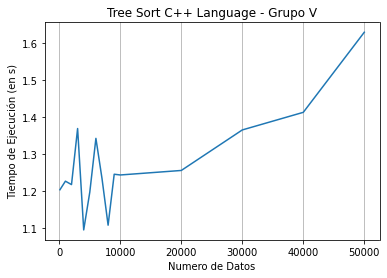
\includegraphics[scale=0.6]{img/treesortcpp.png}
        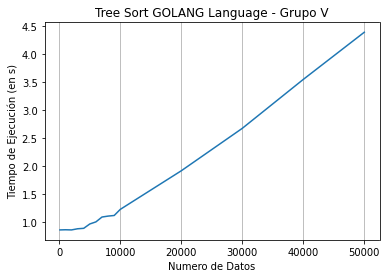
\includegraphics[scale=0.6]{img/treesortgo.png}
        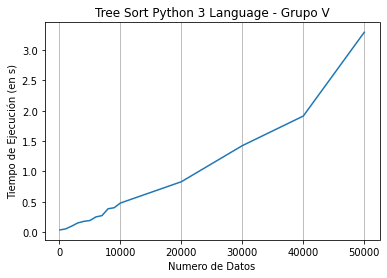
\includegraphics[scale=0.6]{img/treesortpy.png}
        \caption{Algoritmo Treesort}
        \label{fig:my_label}
    \end{figure}

\begin{table}[t]
\begin{center}
\begin{tabular}{| c | c | c | c | c | c | c |}
\hline
\multicolumn{7}{ |c| }{Algoritmo TreeSort - Promedios y Desviacion Estandar} \\ \hline
Datos & C++ (s) & Go (s) & Py (s) &  DE C++ & DE Go & DE Py\\ \hline
100 & 1.203 &0.867 & 0.0348 & 0.03118 & 0.10078 & 0.00295 \\
1000 & 1.2262 & 0.8704 & 0.0504 & 0.11282 & 0.06405 & 0.01013 \\
2000 & 1.227 & 0.8776 & 0.095 & 0.11981 & 0.08759 & 0.02387 \\
3000 & 1.3686 & 0.888 & 0.148 & 0.16048 & 0.13903 &  0.02758 \\
4000 & 1.0944 & 0.8960 & 0.1756 & 0.315517 & 0.078064 & 0.02364 \\
5000 & 1.1968 & 0.9738 & 0.1892 &  0.12132 & 0.13485 & 0.02205 \\
6000 & 1.34 & 1.01 & 0.2488 & 0.157074 & 0.08069 &  0.04511 \\
7000 & 1.2334 & 1.0976 & 0.2708 & 0.10924 & 0.10596 & 0.06994 \\
8000 & 1.1072 & 1.114 & 0.3836 & 0.06894 & 0.12673 & 0.03658 \\
9000 & 1.2449 & 1.125 & 0.4004 & 0.08576 & 0.07631 & 0.02275 \\
10000 & 1.243 & 1.2344 & 0.47 &  0.11511 & 0.12151 & 0.056922 \\
20000 & 1.2551 & 1.923 & 0.8286 & 0.06640 & 0.14278 &  0.1019 \\
30000 & 1.3648 & 2.6802 & 1.4236 &  0.12060 & 0.18089 & 0.117000 \\
40000 & 1.4124 & 3.5530 & 1.9113 & 0.08527 &  0.27471 & 0.14817 \\
50000 & 1.629 & 4.3946 & 3.2928  & 0.10534  &  0.31841 & 0.20671 \\ \hline
\end{tabular}
\caption{Tiempo de Ejecución TreeSort}
\label{tab:coches}
\end{center}
\end{table}

\subsection{Quick Sort}
\begin{figure}[H]
	\centering
	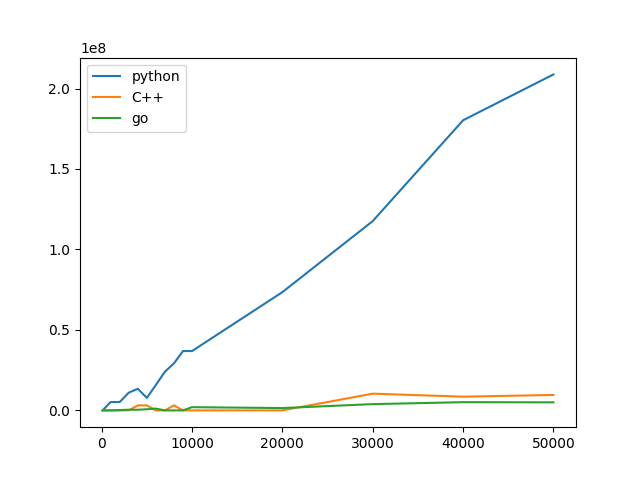
\includegraphics[scale=0.6]{img/quicksort_1.png}
	\caption{Algoritmo Quicksort}
	\label{fig:my_label}
\end{figure}
\newpage
\begin{table}[H]
	\begin{center}
		\begin{tabular}{| c | c | c | c | c | c | c |}
			\hline
			\multicolumn{7}{ |c| }{Algoritmo Quicksort - Promedios y Desviacion Estandar} \\ \hline
			Datos & C++ (ns) & Go (ns) & Py (ns) &  DE C++ & DE Go & DE Py\\ \hline
			100 & 0.0 & 0.0 & 0.0 & 0.0 & 0.0 & 0.0 \\
			1000 & 0.0 & 0.0 & 5208600.0 & 0.0 & 0.0 & 7366072.7 \\
			2000 & 0.0 & 203460.0 & 5207900.0 & 0.0 & 249215.9 & 7365082.8 \\
			3000 & 0.0 & 413200.0 & 11032883.3 & 0.0 & 206604.8 &  7910433.4 \\
			4000 & 3124600.0 & 411640.0 & 13432433.3 & 6249200.0 & 205822.7 & 6074291.9 \\
			5000 & 3124800.0 & 708880.0 & 7811283.3 &  6249600.0 & 1175956.2 & 7811283.4 \\
			6000 & 0.0 & 1105380.0 & 15808183.3 & 0.0 & 2210760.0 &  411578.6 \\
			7000 & 0.0 & 0.0 & 24004683.3 & 0.0 & 0.0 & 8455592.7 \\
			8000 & 3125200.0 & 0.0 & 29220716.6 & 6250400.0 & 0.0 & 10096888.9 \\
			9000 & 0.0 & 0.0 & 36872233.3 & 0.0 & 0.0 & 7126993.4 \\
			10000 & 0.0 & 2006200.0 & 36869583.3 &  0.0 & 4012400.0 & 7981065.8 \\
			20000 & 0.0 & 1453500.0 & 73487433.3 & 0.0 & 763500.2 &  11194532.3 \\
			30000 & 10390400.0 & 3901340.0 & 117625616.6 &  8684150.0 & 3338338.6 & 8302441.4 \\
			40000 & 8522000.0 & 5109060.0 & 180275883.3 & 5014864.0 &  2553783.2 & 14059537.9 \\
			50000 & 9594600.0 & 5011120.0 & 208779083.3  & 489573.5  &  467291.0 & 12087924.9 \\ \hline
		\end{tabular}
		\caption{Tiempo de Ejecución}
		\label{tab:coches}
	\end{center}
\end{table}

\subsection{Heap Sort}
\begin{figure}[H]
	\centering
	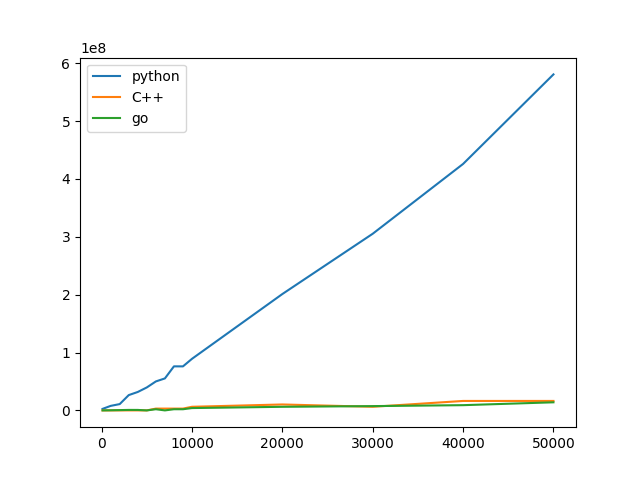
\includegraphics[scale=0.6]{img/heapsort_1.png}
	\caption{Algoritmo Heapsort}
	\label{fig:my_label}
\end{figure}
\newpage
\begin{table}[t]
	\begin{center}
		\begin{tabular}{| c | c | c | c | c | c | c |}
			\hline
			\multicolumn{7}{ |c| }{Algoritmo Heapsort - Promedios y Desviacion Estandar} \\ \hline
			Datos & C++ (s) & Go (s) & Py (s) &  DE C++ & DE Go & DE Py\\ \hline
			100 & 0.0 & 0.0 & 2603950.0 & 0.0 & 0.0 & 5822609.2 \\
			1000 & 0.0 & 206800.0 & 7812200.0 & 0.0 & 253291.1 & 7812200.0 \\
			2000 & 0.0 & 516220.0 & 10905833.3 & 0.0 & 1710.4 & 7781122.6 \\
			3000 & 0.0 & 836680.0 & 26458883.34 & 0.0 & 261797.7 &  7712177.3 \\
			4000 & 0.0 & 813980.0 & 31865516.6 & 0.0 & 516241.5 & 9125481.2 \\
			5000 & 0.0 & 0.0 & 39703883.3 &  0.0 & 0.0 & 8553207.1 \\
			6000 & 3124800.0 & 2006100.0 & 50064733.3 & 6249600.0 & 4012200.0 & 7135993.5 \\
			7000 & 3125000.0 & 0.0 & 55257450.0 & 6250000.0 & 0.0 & 7330155.2 \\
			8000 & 3124800.0 & 2017780.0 & 76115666.6 & 6249600.0 & 4035560.0 & 6229336.5 \\
			9000 & 3125000.0 & 2005460.0 & 76083966.6 & 6250000.0 & 4010920.0 & 6200907.8 \\
			10000 & 6249600.0 & 4026100.0 & 89165300.0 &  7654165.5 & 4931008.7 & 6568716.0 \\
			20000 & 10253200.0 & 6215360.0 & 201116500.0 & 8523860.1 & 1947155.2 &  10964874.8 \\
			30000 & 6250000.0 & 7418220.0 & 305298400.0 & 7654655.4 & 2350517.3 & 14019960.2 \\
			40000 & 16332800.0 & 9045760.0 & 425932733.3333333 & 1416100.4 &  1953907.0 & 12883969.9 \\
			50000 & 16348400.0 & 13987940.0 & 580658700.0  & 1446800.2 & 478307.0 & 35709778.9 \\ \hline
		\end{tabular}
		\caption{Tiempo de Ejecución}
		\label{tab:coches}
	\end{center}
\end{table}

\section{Conclusiones}
    \subsection{Merge Sort} 
    \begin{itemize}
        \item El enguaje C++ utiliza menos tiempo en ejecutar este algoritmo (entre 1 a 2 segundos). Y que, puede ejecutar cargas de millones de datos en tiempos menores. 
        \item El lenguaje Go utiliza similar tiempo con el C++, pero a su vez tiende a aumentar linealmente su tiempo de ejecución. Ambos lenguajes anteriormente mencionados son derivados del C.
        \item Para el lenguaje Python, este muestra un aumento del tiempo exponencial. La razon es sencilla: y es que este lenguaje es interpretado, o sea, mientras compila el programa, ejecuta las funciones. Y por tal para algunos procesamientos de millones de datos puede que no sea tan efectivo.
        \item Interpretando las desviaciones estandar, se tiene que para los lenguajes C++ y Go se tienen variaciones notorias para los analisis de 100 a 10000 datos. En cambio, para Python si se tiene una desviacion estandar bajas debido a que los tiempos de compilacion son altos.
        
    \end{itemize}

    \subsection{Tree Sort}
	\begin{itemize}
        \item El enguaje C++ cuenta con una ejecución mas rápida (entre 1 a 2 segundos, en comparación a los otros lenguajes) razón por la cual se podria observar variaciones en los tiempos de los datos menores.
        \item El lenguaje Go cuenta con una elevacion progresiva relacionada que tiene relacion con la complejidad del algoritmo.
        \item Para el lenguaje Python, este muestra un ligero aumento del tiempo exponencial que en la parte final se podría observar mejor con una mayor cantidad de datos.        
    \end{itemize}

	
	\subsection{Quick Sort}
		\begin{itemize}
			\item El enguaje Go y C++ cuentas con las ejecuciones más rápidas de 0 a 0.1 segundos, se puede observar que apartir de los 20 mil datos el lenguaje Go es más rápido por pequeñas diferencias.
			\item Para el lenguaje Python, este muestra un gran incremento de timepo de ejecución con respecto a los otros dos lenguajes.        
		\end{itemize}
	
	\subsection{Heap Sort}
		\begin{itemize}
			\item El enguaje Go y C++ cuentas con las ejecuciones más rápidas de 0 a 0.1 segundos, se puede observar que apartir de los 30 mil datos el lenguaje Go es más rápido por pequeñas diferencias.
			\item Para el lenguaje Python, este muestra un gran incremento de timepo de ejecución con respecto a los otros dos lenguajes.        
		\end{itemize}
		
	\end{document}
	